\documentclass{standalone}
\usepackage{tikz}
\usetikzlibrary{patterns, positioning}

\begin{document}
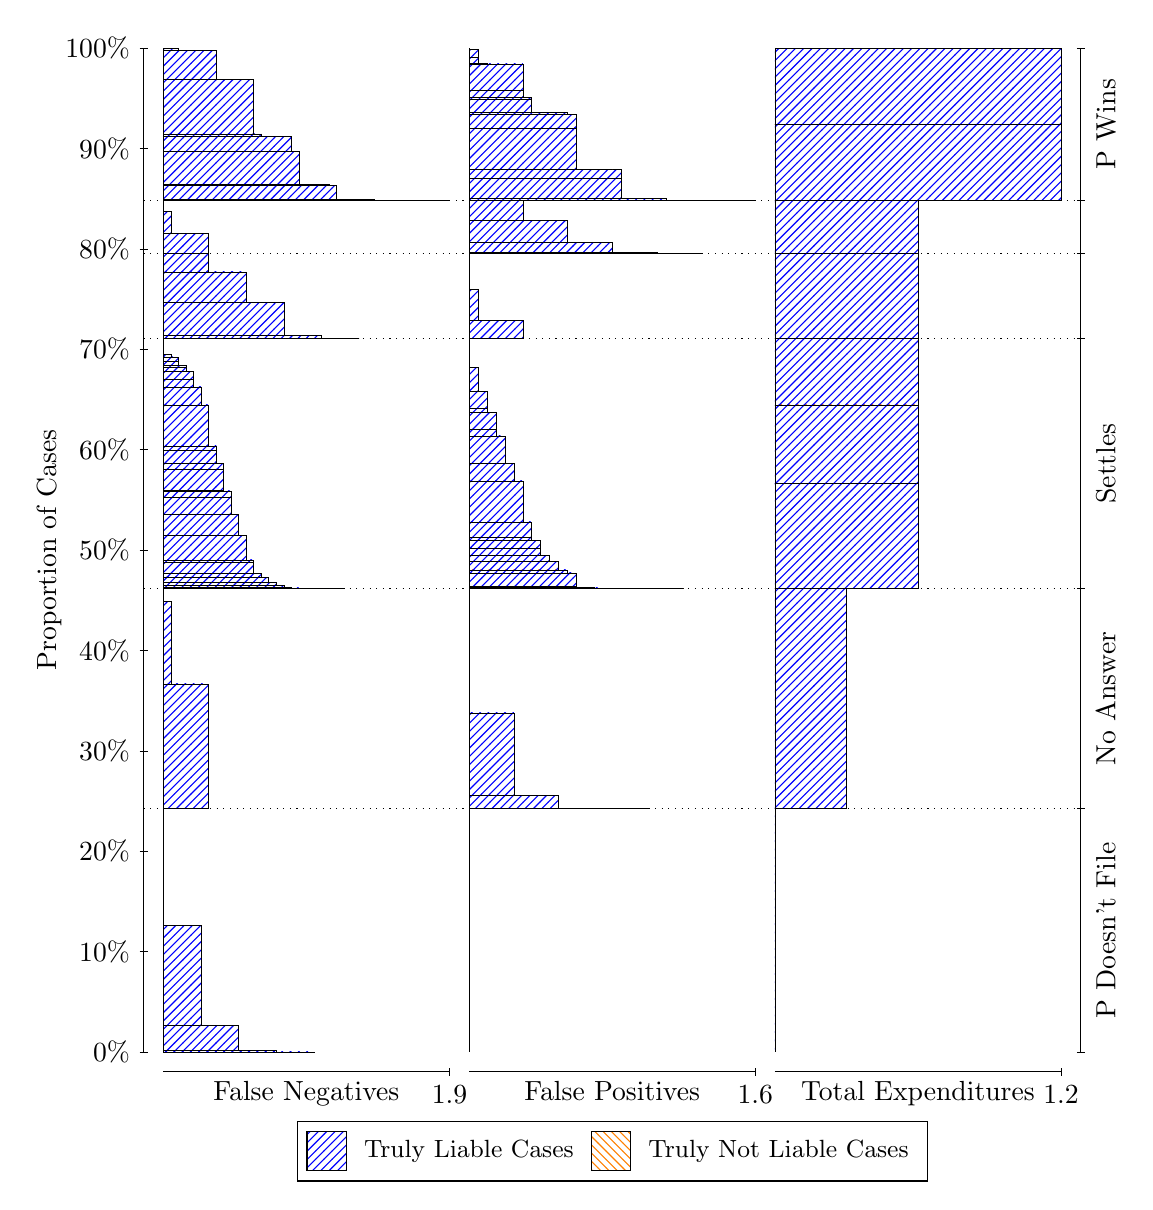
\begin{tikzpicture}
\draw[black, very thin] (1.5,1.75) -- (1.5,14.5);
\node[rotate=90, anchor=center] at (0.3, 8.125) {Proportion of Cases};
\draw[black, very thin] (1.45,1.75) -- (1.55,1.75);
\node[anchor=east] at (1.45, 1.75) {0\%};
\draw[black, very thin] (1.45,3.025) -- (1.55,3.025);
\node[anchor=east] at (1.45, 3.025) {10\%};
\draw[black, very thin] (1.45,4.3) -- (1.55,4.3);
\node[anchor=east] at (1.45, 4.3) {20\%};
\draw[black, very thin] (1.45,5.575) -- (1.55,5.575);
\node[anchor=east] at (1.45, 5.575) {30\%};
\draw[black, very thin] (1.45,6.85) -- (1.55,6.85);
\node[anchor=east] at (1.45, 6.85) {40\%};
\draw[black, very thin] (1.45,8.125) -- (1.55,8.125);
\node[anchor=east] at (1.45, 8.125) {50\%};
\draw[black, very thin] (1.45,9.4) -- (1.55,9.4);
\node[anchor=east] at (1.45, 9.4) {60\%};
\draw[black, very thin] (1.45,10.675) -- (1.55,10.675);
\node[anchor=east] at (1.45, 10.675) {70\%};
\draw[black, very thin] (1.45,11.95) -- (1.55,11.95);
\node[anchor=east] at (1.45, 11.95) {80\%};
\draw[black, very thin] (1.45,13.225) -- (1.55,13.225);
\node[anchor=east] at (1.45, 13.225) {90\%};
\draw[black, very thin] (1.45,14.5) -- (1.55,14.5);
\node[anchor=east] at (1.45, 14.5) {100\%};

\draw[black, very thin] (13.4,1.75) -- (13.4,14.5);
\draw[black, very thin] (13.35,1.75) -- (13.45,1.75);
\node[anchor=west] at (13.35, 1.75) {};
\draw[black, very thin] (13.35,4.8411) -- (13.45,4.8411);
\node[anchor=west] at (13.35, 4.8411) {};
\draw[black, very thin] (13.35,7.6379) -- (13.45,7.6379);
\node[anchor=west] at (13.35, 7.6379) {};
\draw[black, very thin] (13.35,10.811) -- (13.45,10.811);
\node[anchor=west] at (13.35, 10.811) {};
\draw[black, very thin] (13.35,11.891) -- (13.45,11.891);
\node[anchor=west] at (13.35, 11.891) {};
\draw[black, very thin] (13.35,12.563) -- (13.45,12.563);
\node[anchor=west] at (13.35, 12.563) {};
\draw[black, very thin] (13.35,14.5) -- (13.45,14.5);
\node[anchor=west] at (13.35, 14.5) {};

\draw[black, very thin, pattern color=blue, pattern=north east lines] (1.75,1.75) rectangle (3.6623,1.7502);
\draw[black, very thin, pattern color=blue, pattern=north east lines] (1.75,1.7502) rectangle (3.1842,1.77);
\draw[black, very thin, pattern color=blue, pattern=north east lines] (1.75,1.77) rectangle (2.7061,2.0835);
\draw[black, very thin, pattern color=blue, pattern=north east lines] (1.75,2.0835) rectangle (2.2281,3.354);
\draw[black, very thin, pattern color=orange, pattern=north west lines] (1.75,3.354) rectangle (1.75,3.354);
\draw[black, very thin, pattern color=blue, pattern=north east lines] (1.75,3.354) rectangle (1.75,4.8411);
\draw[black, very thin, pattern color=blue, pattern=north east lines] (1.75,4.8411) rectangle (2.3237,6.4237);
\draw[black, very thin, pattern color=blue, pattern=north east lines] (1.75,6.4237) rectangle (1.8456,7.4749);
\draw[black, very thin, pattern color=orange, pattern=north west lines] (1.75,7.4749) rectangle (1.75,7.4749);
\draw[black, very thin, pattern color=blue, pattern=north east lines] (1.75,7.4749) rectangle (1.75,7.6379);
\draw[black, very thin, pattern color=blue, pattern=north east lines] (1.75,7.6379) rectangle (4.0447,7.638);
\draw[black, very thin, pattern color=blue, pattern=north east lines] (1.75,7.638) rectangle (3.8535,7.638);
\draw[black, very thin, pattern color=blue, pattern=north east lines] (1.75,7.638) rectangle (3.6623,7.6403);
\draw[black, very thin, pattern color=blue, pattern=north east lines] (1.75,7.6403) rectangle (3.5667,7.6423);
\draw[black, very thin, pattern color=blue, pattern=north east lines] (1.75,7.6423) rectangle (3.4711,7.6423);
\draw[black, very thin, pattern color=blue, pattern=north east lines] (1.75,7.6423) rectangle (3.4711,7.6448);
\draw[black, very thin, pattern color=blue, pattern=north east lines] (1.75,7.6448) rectangle (3.3754,7.6484);
\draw[black, very thin, pattern color=blue, pattern=north east lines] (1.75,7.6484) rectangle (3.2798,7.6771);
\draw[black, very thin, pattern color=blue, pattern=north east lines] (1.75,7.6771) rectangle (3.1842,7.7115);
\draw[black, very thin, pattern color=blue, pattern=north east lines] (1.75,7.7115) rectangle (3.0886,7.7781);
\draw[black, very thin, pattern color=blue, pattern=north east lines] (1.75,7.7781) rectangle (2.993,7.7823);
\draw[black, very thin, pattern color=blue, pattern=north east lines] (1.75,7.7823) rectangle (2.993,7.8292);
\draw[black, very thin, pattern color=blue, pattern=north east lines] (1.75,7.8292) rectangle (2.8974,7.9632);
\draw[black, very thin, pattern color=blue, pattern=north east lines] (1.75,7.9632) rectangle (2.8974,8);
\draw[black, very thin, pattern color=blue, pattern=north east lines] (1.75,8) rectangle (2.8018,8.3112);
\draw[black, very thin, pattern color=blue, pattern=north east lines] (1.75,8.3112) rectangle (2.7061,8.5729);
\draw[black, very thin, pattern color=blue, pattern=north east lines] (1.75,8.5729) rectangle (2.6105,8.793);
\draw[black, very thin, pattern color=blue, pattern=north east lines] (1.75,8.793) rectangle (2.6105,8.8744);
\draw[black, very thin, pattern color=blue, pattern=north east lines] (1.75,8.8744) rectangle (2.5149,8.8864);
\draw[black, very thin, pattern color=blue, pattern=north east lines] (1.75,8.8864) rectangle (2.5149,9.1553);
\draw[black, very thin, pattern color=blue, pattern=north east lines] (1.75,9.1553) rectangle (2.5149,9.2287);
\draw[black, very thin, pattern color=blue, pattern=north east lines] (1.75,9.2287) rectangle (2.4193,9.3877);
\draw[black, very thin, pattern color=blue, pattern=north east lines] (1.75,9.3877) rectangle (2.4193,9.4466);
\draw[black, very thin, pattern color=blue, pattern=north east lines] (1.75,9.4466) rectangle (2.3237,9.9678);
\draw[black, very thin, pattern color=blue, pattern=north east lines] (1.75,9.9678) rectangle (2.2281,10.197);
\draw[black, very thin, pattern color=blue, pattern=north east lines] (1.75,10.197) rectangle (2.1325,10.296);
\draw[black, very thin, pattern color=blue, pattern=north east lines] (1.75,10.296) rectangle (2.1325,10.391);
\draw[black, very thin, pattern color=blue, pattern=north east lines] (1.75,10.391) rectangle (2.0368,10.393);
\draw[black, very thin, pattern color=blue, pattern=north east lines] (1.75,10.393) rectangle (2.0368,10.443);
\draw[black, very thin, pattern color=blue, pattern=north east lines] (1.75,10.443) rectangle (2.0368,10.466);
\draw[black, very thin, pattern color=blue, pattern=north east lines] (1.75,10.466) rectangle (1.9412,10.518);
\draw[black, very thin, pattern color=blue, pattern=north east lines] (1.75,10.518) rectangle (1.9412,10.577);
\draw[black, very thin, pattern color=blue, pattern=north east lines] (1.75,10.577) rectangle (1.8456,10.613);
\draw[black, very thin, pattern color=orange, pattern=north west lines] (1.75,10.613) rectangle (1.75,10.613);
\draw[black, very thin, pattern color=blue, pattern=north east lines] (1.75,10.613) rectangle (1.75,10.811);
\draw[black, very thin, pattern color=blue, pattern=north east lines] (1.75,10.811) rectangle (4.236,10.811);
\draw[black, very thin, pattern color=blue, pattern=north east lines] (1.75,10.811) rectangle (3.7579,10.85);
\draw[black, very thin, pattern color=blue, pattern=north east lines] (1.75,10.85) rectangle (3.2798,11.27);
\draw[black, very thin, pattern color=blue, pattern=north east lines] (1.75,11.27) rectangle (2.8018,11.657);
\draw[black, very thin, pattern color=blue, pattern=north east lines] (1.75,11.657) rectangle (2.3237,11.891);
\draw[black, very thin, pattern color=orange, pattern=north west lines] (1.75,11.891) rectangle (1.75,11.891);
\draw[black, very thin, pattern color=blue, pattern=north east lines] (1.75,11.891) rectangle (2.3237,12.143);
\draw[black, very thin, pattern color=blue, pattern=north east lines] (1.75,12.143) rectangle (1.8456,12.426);
\draw[black, very thin, pattern color=orange, pattern=north west lines] (1.75,12.426) rectangle (1.75,12.426);
\draw[black, very thin, pattern color=blue, pattern=north east lines] (1.75,12.426) rectangle (1.75,12.563);
\draw[black, very thin, pattern color=blue, pattern=north east lines] (1.75,12.563) rectangle (5.3833,12.563);
\draw[black, very thin, pattern color=blue, pattern=north east lines] (1.75,12.563) rectangle (4.9053,12.563);
\draw[black, very thin, pattern color=blue, pattern=north east lines] (1.75,12.563) rectangle (4.4272,12.582);
\draw[black, very thin, pattern color=blue, pattern=north east lines] (1.75,12.582) rectangle (4.3316,12.582);
\draw[black, very thin, pattern color=blue, pattern=north east lines] (1.75,12.582) rectangle (3.9491,12.759);
\draw[black, very thin, pattern color=blue, pattern=north east lines] (1.75,12.759) rectangle (3.8535,12.766);
\draw[black, very thin, pattern color=blue, pattern=north east lines] (1.75,12.766) rectangle (3.4711,13.189);
\draw[black, very thin, pattern color=blue, pattern=north east lines] (1.75,13.189) rectangle (3.3754,13.376);
\draw[black, very thin, pattern color=blue, pattern=north east lines] (1.75,13.376) rectangle (2.993,13.409);
\draw[black, very thin, pattern color=blue, pattern=north east lines] (1.75,13.409) rectangle (2.8974,14.1);
\draw[black, very thin, pattern color=blue, pattern=north east lines] (1.75,14.1) rectangle (2.5149,14.1);
\draw[black, very thin, pattern color=blue, pattern=north east lines] (1.75,14.1) rectangle (2.4193,14.468);
\draw[black, very thin, pattern color=blue, pattern=north east lines] (1.75,14.468) rectangle (1.9412,14.5);
\draw[black, very thin, pattern color=orange, pattern=north west lines] (1.75,14.5) rectangle (1.75,14.5);
\draw[black, very thin, pattern color=blue, pattern=north east lines] (1.75,14.5) rectangle (1.75,14.5);
\draw[black, very thin, pattern color=orange, pattern=north west lines] (5.6333,1.75) rectangle (5.6333,1.75);
\draw[black, very thin, pattern color=blue, pattern=north east lines] (5.6333,1.75) rectangle (5.6333,4.8411);
\draw[black, very thin, pattern color=orange, pattern=north west lines] (5.6333,4.8411) rectangle (7.9042,4.8411);
\draw[black, very thin, pattern color=blue, pattern=north east lines] (5.6333,4.8411) rectangle (7.9042,4.8411);
\draw[black, very thin, pattern color=blue, pattern=north east lines] (5.6333,4.8411) rectangle (7.3365,4.8419);
\draw[black, very thin, pattern color=blue, pattern=north east lines] (5.6333,4.8419) rectangle (6.7687,5.0041);
\draw[black, very thin, pattern color=blue, pattern=north east lines] (5.6333,5.0041) rectangle (6.201,6.0553);
\draw[black, very thin, pattern color=blue, pattern=north east lines] (5.6333,6.0553) rectangle (5.6333,7.6379);
\draw[black, very thin, pattern color=orange, pattern=north west lines] (5.6333,7.6379) rectangle (8.3583,7.6379);
\draw[black, very thin, pattern color=blue, pattern=north east lines] (5.6333,7.6379) rectangle (8.3583,7.6379);
\draw[black, very thin, pattern color=orange, pattern=north west lines] (5.6333,7.6379) rectangle (8.1313,7.6379);
\draw[black, very thin, pattern color=blue, pattern=north east lines] (5.6333,7.6379) rectangle (8.1313,7.638);
\draw[black, very thin, pattern color=orange, pattern=north west lines] (5.6333,7.638) rectangle (7.9042,7.638);
\draw[black, very thin, pattern color=blue, pattern=north east lines] (5.6333,7.638) rectangle (7.9042,7.638);
\draw[black, very thin, pattern color=blue, pattern=north east lines] (5.6333,7.638) rectangle (7.7906,7.6386);
\draw[black, very thin, pattern color=orange, pattern=north west lines] (5.6333,7.6386) rectangle (7.6771,7.6386);
\draw[black, very thin, pattern color=blue, pattern=north east lines] (5.6333,7.6386) rectangle (7.6771,7.6387);
\draw[black, very thin, pattern color=blue, pattern=north east lines] (5.6333,7.6387) rectangle (7.5635,7.6394);
\draw[black, very thin, pattern color=orange, pattern=north west lines] (5.6333,7.6394) rectangle (7.45,7.6394);
\draw[black, very thin, pattern color=blue, pattern=north east lines] (5.6333,7.6394) rectangle (7.45,7.6396);
\draw[black, very thin, pattern color=blue, pattern=north east lines] (5.6333,7.6396) rectangle (7.3365,7.6429);
\draw[black, very thin, pattern color=orange, pattern=north west lines] (5.6333,7.6429) rectangle (7.2229,7.6429);
\draw[black, very thin, pattern color=blue, pattern=north east lines] (5.6333,7.6429) rectangle (7.2229,7.6485);
\draw[black, very thin, pattern color=blue, pattern=north east lines] (5.6333,7.6485) rectangle (7.1094,7.6542);
\draw[black, very thin, pattern color=blue, pattern=north east lines] (5.6333,7.6542) rectangle (6.9958,7.6624);
\draw[black, very thin, pattern color=orange, pattern=north west lines] (5.6333,7.6624) rectangle (6.9958,7.6624);
\draw[black, very thin, pattern color=blue, pattern=north east lines] (5.6333,7.6624) rectangle (6.9958,7.8354);
\draw[black, very thin, pattern color=blue, pattern=north east lines] (5.6333,7.8354) rectangle (6.8823,7.8718);
\draw[black, very thin, pattern color=orange, pattern=north west lines] (5.6333,7.8718) rectangle (6.7687,7.8718);
\draw[black, very thin, pattern color=blue, pattern=north east lines] (5.6333,7.8718) rectangle (6.7687,7.983);
\draw[black, very thin, pattern color=blue, pattern=north east lines] (5.6333,7.983) rectangle (6.6552,8.0575);
\draw[black, very thin, pattern color=orange, pattern=north west lines] (5.6333,8.0575) rectangle (6.5417,8.0575);
\draw[black, very thin, pattern color=blue, pattern=north east lines] (5.6333,8.0575) rectangle (6.5417,8.1524);
\draw[black, very thin, pattern color=blue, pattern=north east lines] (5.6333,8.1524) rectangle (6.5417,8.2515);
\draw[black, very thin, pattern color=blue, pattern=north east lines] (5.6333,8.2515) rectangle (6.4281,8.2818);
\draw[black, very thin, pattern color=blue, pattern=north east lines] (5.6333,8.2818) rectangle (6.4281,8.481);
\draw[black, very thin, pattern color=blue, pattern=north east lines] (5.6333,8.481) rectangle (6.3146,9.0021);
\draw[black, very thin, pattern color=blue, pattern=north east lines] (5.6333,9.0021) rectangle (6.201,9.2201);
\draw[black, very thin, pattern color=blue, pattern=north east lines] (5.6333,9.2201) rectangle (6.0875,9.5743);
\draw[black, very thin, pattern color=blue, pattern=north east lines] (5.6333,9.5743) rectangle (5.974,9.6557);
\draw[black, very thin, pattern color=blue, pattern=north east lines] (5.6333,9.6557) rectangle (5.974,9.8758);
\draw[black, very thin, pattern color=blue, pattern=north east lines] (5.6333,9.8758) rectangle (5.8604,9.9251);
\draw[black, very thin, pattern color=blue, pattern=north east lines] (5.6333,9.9251) rectangle (5.8604,10.138);
\draw[black, very thin, pattern color=blue, pattern=north east lines] (5.6333,10.138) rectangle (5.7469,10.449);
\draw[black, very thin, pattern color=blue, pattern=north east lines] (5.6333,10.449) rectangle (5.6333,10.811);
\draw[black, very thin, pattern color=orange, pattern=north west lines] (5.6333,10.811) rectangle (6.3146,10.811);
\draw[black, very thin, pattern color=blue, pattern=north east lines] (5.6333,10.811) rectangle (6.3146,11.045);
\draw[black, very thin, pattern color=blue, pattern=north east lines] (5.6333,11.045) rectangle (5.7469,11.432);
\draw[black, very thin, pattern color=blue, pattern=north east lines] (5.6333,11.432) rectangle (5.6333,11.891);
\draw[black, very thin, pattern color=orange, pattern=north west lines] (5.6333,11.891) rectangle (8.5854,11.891);
\draw[black, very thin, pattern color=blue, pattern=north east lines] (5.6333,11.891) rectangle (8.5854,11.892);
\draw[black, very thin, pattern color=blue, pattern=north east lines] (5.6333,11.892) rectangle (8.0177,11.906);
\draw[black, very thin, pattern color=blue, pattern=north east lines] (5.6333,11.906) rectangle (7.45,12.029);
\draw[black, very thin, pattern color=blue, pattern=north east lines] (5.6333,12.029) rectangle (6.8823,12.312);
\draw[black, very thin, pattern color=blue, pattern=north east lines] (5.6333,12.312) rectangle (6.3146,12.563);
\draw[black, very thin, pattern color=orange, pattern=north west lines] (5.6333,12.563) rectangle (9.2667,12.563);
\draw[black, very thin, pattern color=blue, pattern=north east lines] (5.6333,12.563) rectangle (9.2667,12.563);
\draw[black, very thin, pattern color=orange, pattern=north west lines] (5.6333,12.563) rectangle (8.699,12.563);
\draw[black, very thin, pattern color=blue, pattern=north east lines] (5.6333,12.563) rectangle (8.699,12.564);
\draw[black, very thin, pattern color=orange, pattern=north west lines] (5.6333,12.564) rectangle (8.1313,12.564);
\draw[black, very thin, pattern color=blue, pattern=north east lines] (5.6333,12.564) rectangle (8.1313,12.595);
\draw[black, very thin, pattern color=blue, pattern=north east lines] (5.6333,12.595) rectangle (7.5635,12.84);
\draw[black, very thin, pattern color=orange, pattern=north west lines] (5.6333,12.84) rectangle (7.5635,12.84);
\draw[black, very thin, pattern color=blue, pattern=north east lines] (5.6333,12.84) rectangle (7.5635,12.963);
\draw[black, very thin, pattern color=orange, pattern=north west lines] (5.6333,12.963) rectangle (7.45,12.963);
\draw[black, very thin, pattern color=blue, pattern=north east lines] (5.6333,12.963) rectangle (7.45,12.963);
\draw[black, very thin, pattern color=blue, pattern=north east lines] (5.6333,12.963) rectangle (6.9958,13.486);
\draw[black, very thin, pattern color=blue, pattern=north east lines] (5.6333,13.486) rectangle (6.9958,13.654);
\draw[black, very thin, pattern color=orange, pattern=north west lines] (5.6333,13.654) rectangle (6.8823,13.654);
\draw[black, very thin, pattern color=blue, pattern=north east lines] (5.6333,13.654) rectangle (6.8823,13.687);
\draw[black, very thin, pattern color=blue, pattern=north east lines] (5.6333,13.687) rectangle (6.4281,13.852);
\draw[black, very thin, pattern color=blue, pattern=north east lines] (5.6333,13.852) rectangle (6.4281,13.874);
\draw[black, very thin, pattern color=blue, pattern=north east lines] (5.6333,13.874) rectangle (6.3146,13.966);
\draw[black, very thin, pattern color=orange, pattern=north west lines] (5.6333,13.966) rectangle (6.3146,13.966);
\draw[black, very thin, pattern color=blue, pattern=north east lines] (5.6333,13.966) rectangle (6.3146,14.298);
\draw[black, very thin, pattern color=blue, pattern=north east lines] (5.6333,14.298) rectangle (5.8604,14.302);
\draw[black, very thin, pattern color=blue, pattern=north east lines] (5.6333,14.302) rectangle (5.8604,14.304);
\draw[black, very thin, pattern color=blue, pattern=north east lines] (5.6333,14.304) rectangle (5.7469,14.378);
\draw[black, very thin, pattern color=blue, pattern=north east lines] (5.6333,14.378) rectangle (5.7469,14.481);
\draw[black, very thin, pattern color=blue, pattern=north east lines] (5.6333,14.481) rectangle (5.6333,14.5);
\draw[black, very thin, pattern color=orange, pattern=north west lines] (9.5167,1.75) rectangle (9.5167,1.75);
\draw[black, very thin, pattern color=blue, pattern=north east lines] (9.5167,1.75) rectangle (9.5167,4.8411);
\draw[black, very thin, pattern color=orange, pattern=north west lines] (9.5167,4.8411) rectangle (10.425,4.8411);
\draw[black, very thin, pattern color=blue, pattern=north east lines] (9.5167,4.8411) rectangle (10.425,7.6379);
\draw[black, very thin, pattern color=orange, pattern=north west lines] (9.5167,7.6379) rectangle (11.333,7.6379);
\draw[black, very thin, pattern color=blue, pattern=north east lines] (9.5167,7.6379) rectangle (11.333,8.9728);
\draw[black, very thin, pattern color=orange, pattern=north west lines] (9.5167,8.9728) rectangle (11.333,8.9728);
\draw[black, very thin, pattern color=blue, pattern=north east lines] (9.5167,8.9728) rectangle (11.333,9.9681);
\draw[black, very thin, pattern color=orange, pattern=north west lines] (9.5167,9.9681) rectangle (11.333,9.9681);
\draw[black, very thin, pattern color=blue, pattern=north east lines] (9.5167,9.9681) rectangle (11.333,10.811);
\draw[black, very thin, pattern color=orange, pattern=north west lines] (9.5167,10.811) rectangle (11.333,10.811);
\draw[black, very thin, pattern color=blue, pattern=north east lines] (9.5167,10.811) rectangle (11.333,11.891);
\draw[black, very thin, pattern color=orange, pattern=north west lines] (9.5167,11.891) rectangle (11.333,11.891);
\draw[black, very thin, pattern color=blue, pattern=north east lines] (9.5167,11.891) rectangle (11.333,12.563);
\draw[black, very thin, pattern color=orange, pattern=north west lines] (9.5167,12.563) rectangle (13.15,12.563);
\draw[black, very thin, pattern color=blue, pattern=north east lines] (9.5167,12.563) rectangle (13.15,13.533);
\draw[black, very thin, pattern color=orange, pattern=north west lines] (9.5167,13.533) rectangle (13.15,13.533);
\draw[black, very thin, pattern color=blue, pattern=north east lines] (9.5167,13.533) rectangle (13.15,14.5);
\draw[black, dotted] (1.5,4.8411) -- (13.4,4.8411);
\draw[black, dotted] (1.5,7.6379) -- (13.4,7.6379);
\draw[black, dotted] (1.5,10.811) -- (13.4,10.811);
\draw[black, dotted] (1.5,11.891) -- (13.4,11.891);
\draw[black, dotted] (1.5,12.563) -- (13.4,12.563);
\draw[black, very thin] (1.75,1.5) -- (5.3833,1.5);
\node[anchor=north] at (3.5667, 1.5) {False Negatives};
\draw[black, very thin] (5.3833,1.45) -- (5.3833,1.55);
\node[anchor=north] at (5.3833, 1.45) {1.9};

\draw[black, very thin] (5.6333,1.5) -- (9.2667,1.5);
\node[anchor=north] at (7.45, 1.5) {False Positives};
\draw[black, very thin] (9.2667,1.45) -- (9.2667,1.55);
\node[anchor=north] at (9.2667, 1.45) {1.6};

\draw[black, very thin] (9.5167,1.5) -- (13.15,1.5);
\node[anchor=north] at (11.333, 1.5) {Total Expenditures};
\draw[black, very thin] (13.15,1.45) -- (13.15,1.55);
\node[anchor=north] at (13.15, 1.45) {1.2};

\node[black, centered, rotate=90] at (13.72, 3.2955) {P Doesn't File};
\node[black, centered, rotate=90] at (13.72, 6.2395) {No Answer};
\node[black, centered, rotate=90] at (13.72, 9.2244) {Settles};


\node[black, centered, rotate=90] at (13.72, 13.532) {P Wins};

\draw (7.449999999999999,1.5) node[draw=none] (baseCoordinate) {};
\begin{scope}[align=center]
        \matrix[scale=0.5, draw=black, below=0.5cm of baseCoordinate, nodes={draw}, column sep=0.1cm]{
            \node[rectangle, draw, minimum width=0.5cm, minimum height=0.5cm, pattern=north east lines, pattern color=blue] {}; &
            \node[draw=none, font=\small] (B) {Truly Liable Cases}; &
            \node[rectangle, draw, minimum width=0.5cm, minimum height=0.5cm, pattern=north west lines, pattern color=orange] {}; &
            \node[draw=none, font=\small] (B) {Truly Not Liable Cases}; \\
            };
\end{scope}

\end{tikzpicture}
\end{document}